\documentclass[a4paper,12pt]{article}

% Paquetes básicos
\usepackage[utf8]{inputenc}
\usepackage[T1]{fontenc}
\usepackage[spanish]{babel}
\usepackage{graphicx}
\usepackage{xcolor}
\usepackage{lipsum}
\usepackage{geometry}
\geometry{top=3cm, bottom=3cm, left=2.5cm, right=2.5cm}
\usepackage{pifont}
\usepackage{array}
\newcolumntype{L}[1]{>{\raggedright\arraybackslash}p{#1}}



% Paquetes para figuras
\usepackage{tikz}
\usetikzlibrary{positioning, arrows}
\usetikzlibrary{positioning, shapes.geometric, decorations.pathreplacing, arrows.meta}

% Define styles for the diagram
\tikzstyle{class} = [rectangle, draw, fill=blue!10, rounded corners, minimum height=2em, minimum width=4cm, text centered]
\tikzstyle{arrow} = [thick, ->, >=stealth]

% Paquetes para diseño
\usepackage{titlesec}
\usepackage{fancyhdr}
\usepackage{amsmath}
\usepackage{amssymb}
\usepackage{hyperref}

% Paquetes para el entorno lstlisting
\usepackage{listings}
\usepackage{inconsolata}

%encabezado y pie de página nivel profesional
\usepackage{fancyhdr}
\pagestyle{fancy}
\fancyhf{}
\fancyhead[L]{\leftmark}
\fancyhead[R]{\rightmark}
\fancyfoot[L]{\textbf{Ismael Sallami Moreno - GIIADE}}
\fancyfoot[C]{\thepage}
\fancyfoot[R]{\textbf{(UGR)} \today}
\renewcommand{\headrulewidth}{0.4pt}
\renewcommand{\footrulewidth}{0.4pt}
\setlength{\headheight}{15pt}
\setlength{\headsep}{10pt}
\setlength{\footskip}{20pt}
\usepackage{truncate}
\fancyhead[L]{\truncate{0.5\headwidth}{\leftmark}}
\fancyhead[R]{\truncate{0.5\headwidth}{\rightmark}}
\usepackage{mathpazo}
\usepackage{tcolorbox}


% Paquete para fondo
\usepackage{background}
\usepackage{float}

% Configuración de lstlisting
\lstset{
    inputencoding=utf8,          % Permite UTF-8
    extendedchars=true,          % Reconoce caracteres extendidos
    literate=                    % Configuración manual para tildes y símbolos
        {á}{{\'a}}1
        {é}{{\'e}}1
        {í}{{\'i}}1
        {ó}{{\'o}}1
        {ú}{{\'u}}1
        {ñ}{{\~n}}1
        {Á}{{\'A}}1
        {É}{{\'E}}1
        {Í}{{\'I}}1
        {Ó}{{\'O}}1
        {Ú}{{\'U}}1
        {Ñ}{{\~N}}1
        {¿}{{\textquestiondown}}1
        {¡}{{\textexclamdown}}1,
    basicstyle=\ttfamily,        % Fuente monoespaciada
    breaklines=true,             % Habilita salto de línea automático
    frame=single,                % Marco alrededor del código
    backgroundcolor=\color{gray!10}, % Fondo gris claro
    keywordstyle=\color{blue},   % Color para palabras clave
    commentstyle=\color{green},  % Color para comentarios
    stringstyle=\color{red}      % Color para strings
}
\lstdefinestyle{customcpp}{
    language=C++,                % Lenguaje de programación
    showspaces=false,            % No mostrar espacios
    showtabs=false,              % No mostrar tabulaciones
    tabsize=4,                   % Tamaño de tabulación
    showstringspaces=false,      % No mostrar espacios en strings
    numbers=left,                % Números de línea a la izquierda
    numberstyle=\tiny\color{gray}, % Estilo de los números de línea
    numbersep=5pt,               % Separación de los números de línea
    stepnumber=1,                % Mostrar número en cada línea
    basicstyle=\ttfamily\footnotesize, % Estilo básico del código
    keywordstyle=\bfseries\color{blue}, % Estilo de las palabras clave
    commentstyle=\itshape\color{green!50!black}, % Estilo de los comentarios
    stringstyle=\color{red},     % Estilo de los strings
    identifierstyle=\color{black}, % Estilo de los identificadores
    % procnamekeys={def,class},    % Palabras clave para nombres de funciones
    morekeywords={constexpr,nullptr,size_t}, % Más palabras clave
    emph={int,char,double,float,unsigned}, % Palabras a enfatizar
    emphstyle=\color{magenta},   % Estilo de las palabras enfatizadas
    backgroundcolor=\color{gray!10}, % Color de fondo
    frame=shadowbox,             % Marco con sombra
    rulesepcolor=\color{gray},   % Color de la línea de separación
    breakatwhitespace=false,     % No cortar en espacios en blanco
    breaklines=true,             % Cortar líneas largas
    captionpos=b,                % Posición del título (abajo)
    escapeinside={(*@}{@*)},     % Delimitadores para escapar a LaTeX
    morecomment=[l][\color{magenta}]{\#}, % Comentarios de una línea
    morecomment=[s][\color{orange}]{/*}{*/}, % Comentarios multilínea
    morestring=[b]",             % Strings entre comillas dobles
    morestring=[b]'              % Strings entre comillas simples
}
\lstdefinestyle{customjava}{
    language=Java,               % Lenguaje de programación
    showspaces=false,            % No mostrar espacios
    showtabs=false,              % No mostrar tabulaciones
    tabsize=4,                   % Tamaño de tabulación
    showstringspaces=false,      % No mostrar espacios en strings
    numbers=left,                % Números de línea a la izquierda
    numberstyle=\tiny\color{gray}, % Estilo de los números de línea
    numbersep=5pt,               % Separación de los números de línea
    stepnumber=1,                % Mostrar número en cada línea
    basicstyle=\ttfamily\footnotesize, % Estilo básico del código
    keywordstyle=\bfseries\color{purple}, % Estilo de las palabras clave
    commentstyle=\itshape\color{green!50!black}, % Estilo de los comentarios
    stringstyle=\color{orange},  % Estilo de los strings
    identifierstyle=\color{black}, % Estilo de los identificadores
    morekeywords={abstract, assert, boolean, break, byte, case, catch, char, class, const, continue, default, do, double, else, enum, extends, final, finally, float, for, goto, if, implements, import, instanceof, int, interface, long, native, new, null, package, private, protected, public, return, short, static, strictfp, super, switch, synchronized, this, throw, throws, transient, try, void, volatile, while}, % Más palabras clave
    emph={int,char,double,float,unsigned}, % Palabras a enfatizar
    emphstyle=\color{magenta},   % Estilo de las palabras enfatizadas
    backgroundcolor=\color{gray!10}, % Color de fondo
    frame=shadowbox,             % Marco con sombra
    rulesepcolor=\color{gray},   % Color de la línea de separación
    breakatwhitespace=false,     % No cortar en espacios en blanco
    breaklines=true,             % Cortar líneas largas
    captionpos=b,                % Posición del título (abajo)
    escapeinside={(*@}{@*)},     % Delimitadores para escapar a LaTeX
    morecomment=[l][\color{magenta}]{\#}, % Comentarios de una línea
    morecomment=[s][\color{orange}]{/*}{*/}, % Comentarios multilínea
    morestring=[b]",             % Strings entre comillas dobles
    morestring=[b]'              % Strings entre comillas simples
}

\lstdefinestyle{customrb}{
    language=Ruby,               % Lenguaje de programación
    showspaces=false,            % No mostrar espacios
    showtabs=false,              % No mostrar tabulaciones
    tabsize=2,                   % Tamaño de tabulación
    showstringspaces=false,      % No mostrar espacios en strings
    numbers=left,                % Números de línea a la izquierda
    numberstyle=\tiny\color{gray}, % Estilo de los números de línea
    numbersep=5pt,               % Separación de los números de línea
    stepnumber=1,                % Mostrar número en cada línea
    basicstyle=\ttfamily\footnotesize, % Estilo básico del código
    keywordstyle=\bfseries\color{blue}, % Estilo de las palabras clave
    commentstyle=\itshape\color{green!50!black}, % Estilo de los comentarios
    stringstyle=\color{red},     % Estilo de los strings
    identifierstyle=\color{black}, % Estilo de los identificadores
    morekeywords={alias, and, BEGIN, begin, break, case, class, def, defined?, do, else, elsif, END, end, ensure, false, for, if, in, module, next, nil, not, or, redo, rescue, retry, return, self, super, then, true, undef, unless, until, when, while, yield}, % Más palabras clave
    emph={int,char,double,float,unsigned}, % Palabras a enfatizar
    emphstyle=\color{magenta},   % Estilo de las palabras enfatizadas
    backgroundcolor=\color{gray!10}, % Color de fondo
    frame=shadowbox,             % Marco con sombra
    rulesepcolor=\color{gray},   % Color de la línea de separación
    breakatwhitespace=false,     % No cortar en espacios en blanco
    breaklines=true,             % Cortar líneas largas
    captionpos=b,                % Posición del título (abajo)
    escapeinside={(*@}{@*)},     % Delimitadores para escapar a LaTeX
    morecomment=[l][\color{magenta}]{\#}, % Comentarios de una línea
    morecomment=[s][\color{orange}]{=begin}{=end}, % Comentarios multilínea
    morestring=[b]",             % Strings entre comillas dobles
    morestring=[b]'              % Strings entre comillas simples
}

% Configuración de título
\titleformat{\section}{\normalfont\Large\bfseries}{\thesection}{1em}{}

% Información del documento
\title{
    \vspace{-2cm}
    
\includegraphics[width=0.3\textwidth]{images/etsiit.png} \\ % Cambia el logo si es necesario
    \LARGE Ingeniería Informática + ADE\\
    \large Universidad de Granada (UGR)\\[1cm]
}
\author{\textbf{Autor:} Ismael Sallami Moreno}
\date{\textbf{Asignatura:} Relación de Problemas Tema 3 : Herencia (PDOO)\\[1cm]}

% Configuración del fondo
\backgroundsetup{
    scale=1,
    color=black,
    opacity=0.2,
    angle=0,
    position=current page.south,
    vshift=0pt,
    hshift=0pt,
    contents={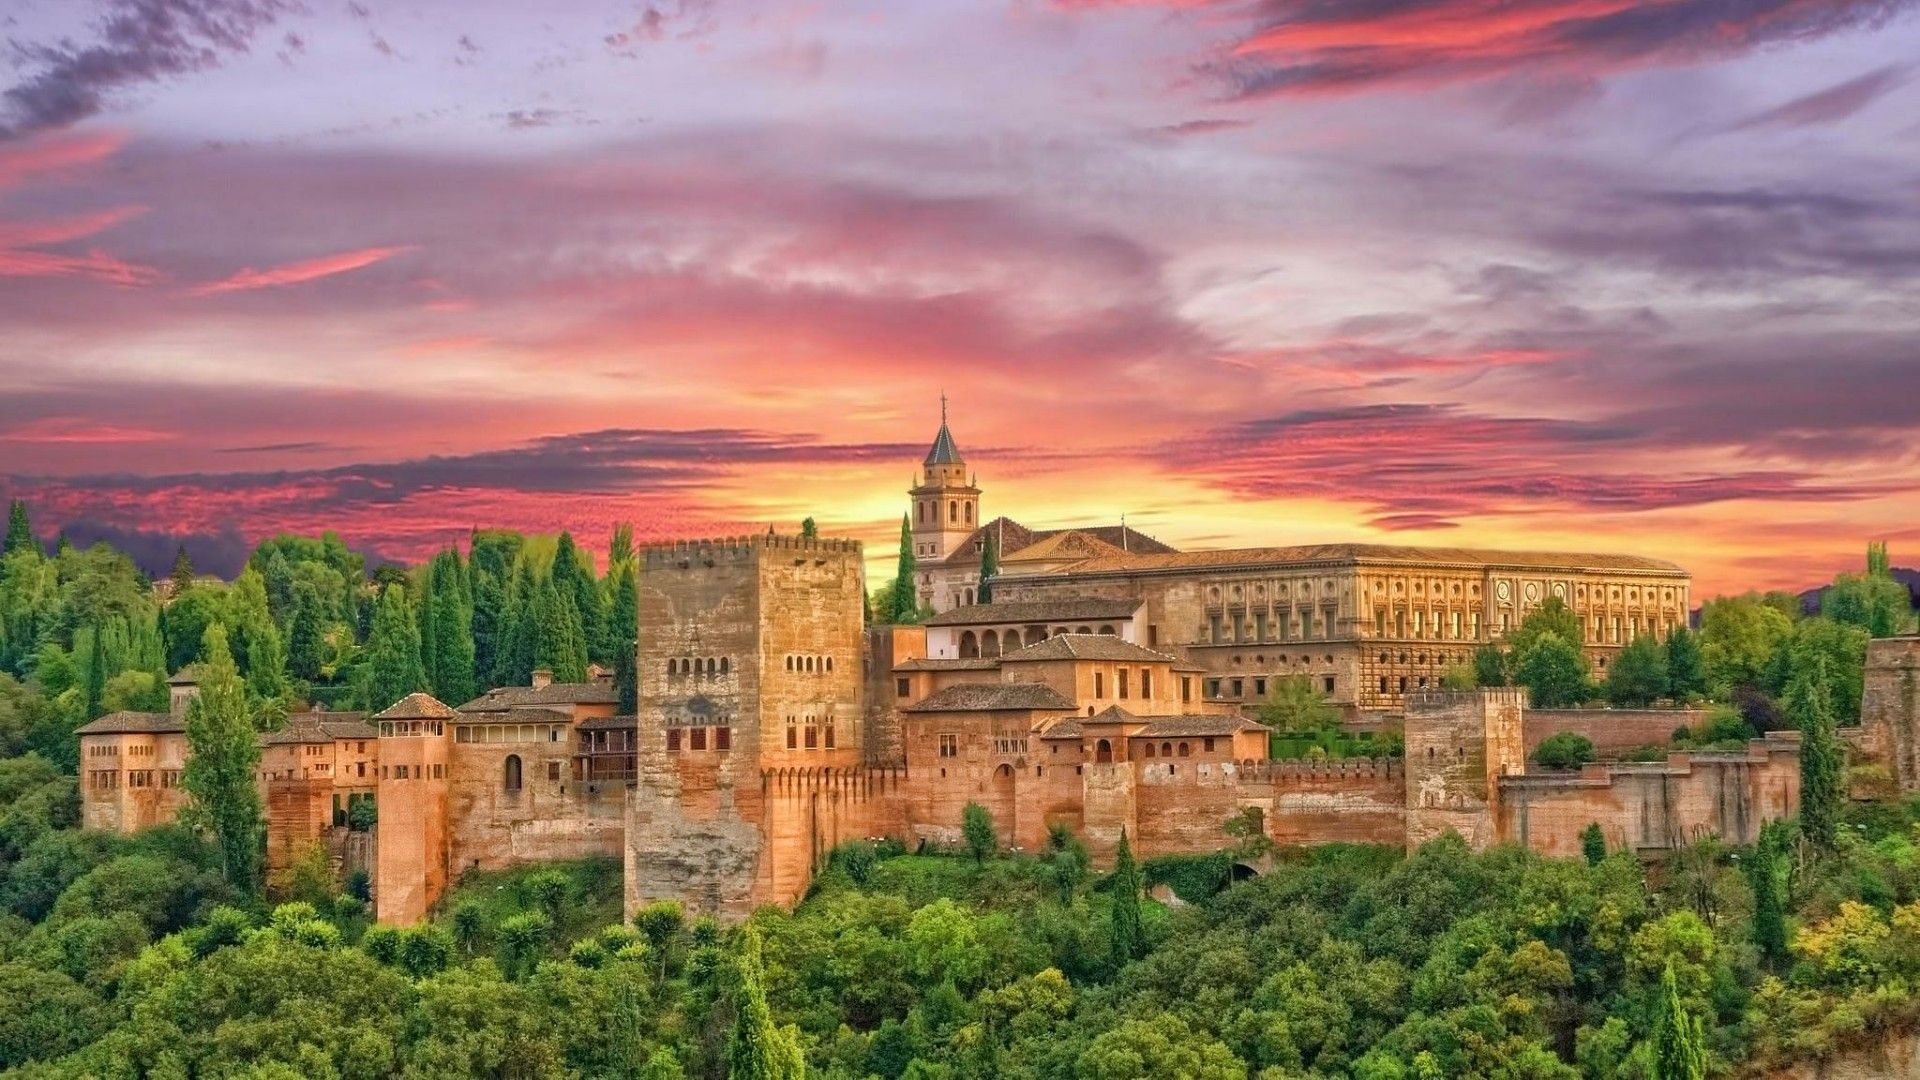
\includegraphics[width=\paperwidth,height=\paperheight,keepaspectratio]{images/granada.jpg}}
}

\usetikzlibrary{positioning}

% Inicio del documento
\begin{document}

% Portada
\maketitle
\thispagestyle{empty}

\begin{center}
    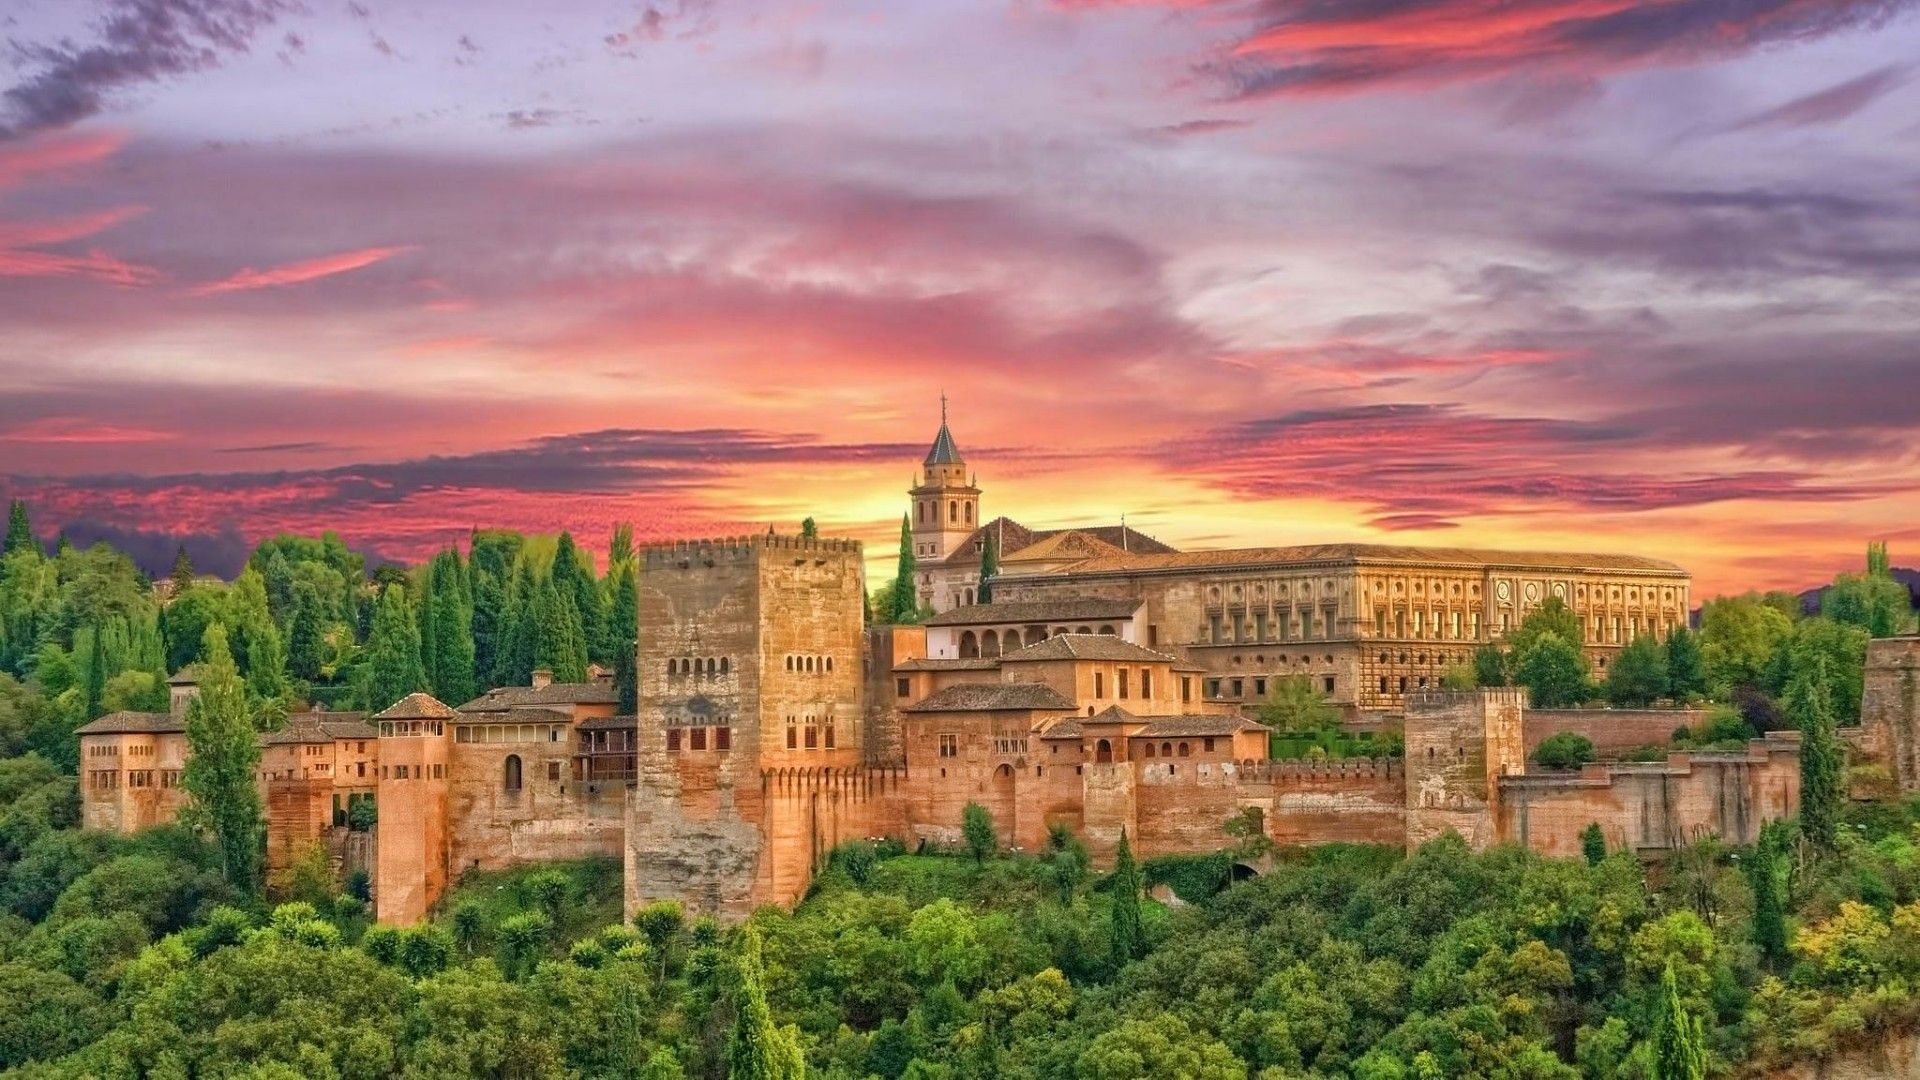
\includegraphics[width=\textwidth,height=0.4\textheight,keepaspectratio]{images/granada.jpg} \\ % Añade tu imagen de fondo
    \vfill
\end{center}

\newpage

% Índice (opcional)
\tableofcontents
\newpage

\section{Ejercicio 1}
\subsection{Enunciado}




Dada la siguiente clase en Java:

\begin{lstlisting}[style=customjava]
public class Vertebrado
{
    public ArrayList<String> partesDelAbdomen();
    public void desplazarse();
    public String comunicarse(Vertebrado vertebrado);
    protected Vertebrado obtenerCopia();
}
\end{lstlisting}

Indica con una cruz en la casilla correspondiente según si la declaración de los siguientes métodos de la clase \texttt{Mamifero}, subclase de \texttt{Vertebrado}, sobrecargan (\emph{overloading}) o redefinen (\emph{overriding}) a los de la clase \texttt{Vertebrado}.

\subsection{Solución}


\begin{table}[H]
    \centering
    \begin{tabular}{|l|c|c|}
    \hline
    \textbf{Método} & \textbf{Sobrecarga} & \textbf{Redefinición} \\ \hline
    public ArrayList<String> partesDelAbdomen() &  & X \\ \hline
    public void desplazarse(Modo m) & X &  \\ \hline
    public String comunicarse(Vertebrado vertebrado) &  & X \\ \hline
    public String comunicarse(Mamifero mamifero) & X &  \\ \hline
    public Vertebrado obtenerCopia() &  & X \\ \hline
    protected Mamifero obtenerCopia() &  & X \\ \hline
    \end{tabular}
\end{table}

\textit{Nota:Al cambiar únicamente la visibilidad o el tipo hace que sea una redefición (Últimos dos casos)}
    

\section{Ejercicio 2}
\subsection{Enunciado}




A partir de las siguientes clases:

\begin{lstlisting}[style=customjava]
public class Persona {
    protected String nombre;
    public Persona(String nom) { this.setNombre(nom); }
    protected String getNombre() { return this.nombre; }
    public String hablar() { return "bla bla bla"; }
}
\end{lstlisting}

\begin{lstlisting}[style=customjava]
public class Estudiante extends Persona {
    public String carrera;
    public int curso;
    public Estudiante(String nom, String carr, int cur) {
        super(nom);
        carrera = carr;
        curso = cur;
    }
    public void estudiar() { System.out.println("Estudiando"); }
}
\end{lstlisting}

Implementa la clase \texttt{EstudianteInformatica} que hereda de \texttt{Estudiante}. Debe tener:

\begin{itemize}
    \item Una nueva variable de instancia que es una colección de \texttt{String} con los dispositivos que utiliza (por ejemplo, \texttt{PC}, \texttt{tablet}, \texttt{smartphone}).
    \item Métodos para consultar esa variable.
    \item Una redefinición del método \texttt{estudiar()} para que además de estudiar como los otros alumnos, diga que estudia con el último dispositivo de su colección.
    \item Un constructor para inicializar la clase.
\end{itemize}

Implementa este problema en Java y Ruby:

% \textbf{Implementación en Java:}

% \begin{lstlisting}[style=customjava]
% public class EstudianteInformatica extends Estudiante {
%     private ArrayList<String> dispositivos;

%     public EstudianteInformatica(String nom, String carr, int cur, ArrayList<String> dispositivos) {
%         super(nom, carr, cur);
%         this.dispositivos = dispositivos;
%     }

%     public ArrayList<String> getDispositivos() {
%         return this.dispositivos;
%     }

%     @Override
%     public void estudiar() {
%         super.estudiar();
%         if (!dispositivos.isEmpty()) {
%             System.out.println("Estudiando con " + dispositivos.get(dispositivos.size() - 1));
%         }
%     }
% }
% \end{lstlisting}

% \textbf{Implementación en Ruby:}

% \begin{lstlisting}[style=customrb]
% class Persona
%     attr_accessor :nombre

%     def initialize(nombre)
%         @nombre = nombre
%     end

%     def hablar
%         "bla bla bla"
%     end
% end

% class Estudiante < Persona
%     attr_accessor :carrera, :curso

%     def initialize(nombre, carrera, curso)
%         super(nombre)
%         @carrera = carrera
%         @curso = curso
%     end

%     def estudiar
%         puts "estudiando"
%     end
% end

% class EstudianteInformatica < Estudiante
%     attr_accessor :dispositivos

%     def initialize(nombre, carrera, curso, dispositivos)
%         super(nombre, carrera, curso)
%         @dispositivos = dispositivos
%     end

%     def estudiar
%         super
%         puts "Estudiando con #{@dispositivos.last}" unless @dispositivos.empty?
%     end
% end
% \end{lstlisting}

\subsection{Solución}

\begin{lstlisting}[style=customjava, caption={Clase Estudiante de Informática}]
    public class EstudianteInformatica extends Estudiante {
        private ArrayList<String> dispositivos;
        public EstudianteInformatica(string nombre, string curso){
            super(nombre, "Informatica", curso);
            dispositivos = new ArrayList<String>();
        }

        @Override
        public void Estudiar(){
            System.out.println("Informatica con " + dispositivos.get(dispositivos.size() - 1));
        }
    } // Fin de la clase EstudianteInformatica
    
\end{lstlisting}

\begin{lstlisting}[style=customrb, caption={Clase Estudiante de Informática}]
    def EstudianteInformatica < Estudiante 
        def initialize (nombre, curso)
            super(nombre, "Informatica", curso)
            @dispositivos = [] # @dispositivos = Array.new
        end

        def Estudiar
            super.Estudiar
            puts "Estudiando Informatica con #{@dispositivos[-1]}"
        end
    end


\end{lstlisting}


\section{Ejercicio 3 }
\subsection{Enunciado}


\textit{Nota: En las diapositivas de la Relación hay un error, donde pone 3, no es el ejercicio 3 es la parte 2 del ejercicio 2, es decir, otra clase, el ejercicio 3 es el marcado con el número 4.}


Dada la siguiente clase abstracta en Java:

\begin{lstlisting}[style=customjava]
abstract class Transporte {
    protected String marca;

    protected String getMarca() {
        return this.marca;
    }

    protected void setMarca(String marc) {
        this.marca = marc;
    }

    public abstract String hacerRuta(String origen, String destino);
}
\end{lstlisting}

Crea dos nuevas clases, \texttt{Bicicleta} y \texttt{NaveEspacial}, que hereden de \texttt{Transporte} e implementen el método \texttt{hacerRuta} de forma diferente:

\subsection{Solución}


\begin{lstlisting}[style=customjava, caption={Clase Bicicleta y Clase Nave Espacial}]
    public class Bicicleta extends Transporte {
        @Override
        public String hacerRuta(String origen, String destino) {
            return "Pedaleando desde " + origen + " hasta " + destino;
        }
    }

    
    public class NaveEspacial extends Transporte {
        @Override
        public String hacerRuta(String origen, String destino) {
            return "Volando desde " + origen + " hasta " + destino + " por el espacio";
        }
    }
    
\end{lstlisting}

\subsection*{Diagrama UML}

\begin{center}
\begin{tikzpicture}[node distance=2.5cm, auto]

% Main class
\node[class] (Transporte) {\textbf{Transporte}};

% Subclasses
\node[class, below left=1.5cm and 1.5cm of Transporte] (Bicicleta) {\textbf{Bicicleta}};
\node[class, below right=1.5cm and 1.5cm of Transporte] (NaveEspacial) {\textbf{NaveEspacial}};

% Arrows
\draw[arrow] (Bicicleta.north) -- (Transporte.south west);
\draw[arrow] (NaveEspacial.north) -- (Transporte.south east);

\end{tikzpicture}
\end{center}

\section{Ejercicio 4} 
\subsection{Enunciado}
Hacer el ejercicio anterior, pero en Ruby.
\subsection{Solución}


\begin{lstlisting}[style=customrb, caption={Clase Bicicleta y Clase Nave Espacial}]
    def Bicicleta < Transporte 
        def hacerRuta(origen, destino)
            "Pedaleando desde #{origen} hasta #{destino}"
        end
    end

    def NaveEspacial < Transporte 
        def hacerRuta(origen, destino)
            "Volando desde #{origen} hasta #{destino} por el espacio"
        end
    end
\end{lstlisting}

\section{Ejercicio 5}

\subsection{Enunciado}

Implementa en Java una clase paramétrica a partir de la cual se puedan definir clases de grupos de personas con un líder, como por ejemplo grupos de música con un cantante, o empresas con un jefe. Implementa también alguna de esas clases a partir de la clase paramétrica definida.

\subsection{Solución}

A continuación, se implementa una clase paramétrica en Java para definir grupos de personas con un líder. Posteriormente, se muestra un ejemplo de uso creando un grupo de música con un cantante.

\begin{lstlisting}[style=customjava]
// Clase paramétrica genérica
public class Grupo<T> {
    private T lider;
    private List<T> miembros;

    public Grupo(T lider) {
        this.lider = lider;
        this.miembros = new ArrayList<>();
    }

    public T getLider() {
        return lider;
    }

    public void setLider(T lider) {
        this.lider = lider;
    }

    public void agregarMiembro(T miembro) {
        this.miembros.add(miembro);
    }

    public List<T> getMiembros() {
        return miembros;
    }

    @Override
    public String toString() {
        return "Líder: " + lider + ", Miembros: " + miembros;
    }
}

// Ejemplo de uso con un grupo de música
public class Musico {
    private String nombre;

    public Musico(String nombre) {
        this.nombre = nombre;
    }

    @Override
    public String toString() {
        return nombre;
    }
}

public class Main {
    public static void main(String[] args) {
        Musico cantante = new Musico("Freddie Mercury");
        Grupo<Musico> banda = new Grupo<>(cantante);
        
        banda.agregarMiembro(new Musico("Brian May"));
        banda.agregarMiembro(new Musico("Roger Taylor"));
        banda.agregarMiembro(new Musico("John Deacon"));

        System.out.println(banda);
    }
}
\end{lstlisting}

Si queremos implementar esta misma solución en Ruby, sería como sigue:

\begin{lstlisting}[style=customrb]
# Clase paramétrica genérica
class Grupo
  attr_accessor :lider, :miembros

  def initialize(lider)
    @lider = lider
    @miembros = []
  end

  def agregar_miembro(miembro)
    @miembros << miembro
    # Otras formas de añadir un miembro en Ruby
    # @miembros.push(miembro)
    # @miembros += [miembro]
    # @miembros.concat([miembro])
  end

  def to_s
    "Líder: #{@lider}, Miembros: #{@miembros.join(', ')}"
  end
end

# Ejemplo de uso con un grupo de música
class Musico
  attr_accessor :nombre

  def initialize(nombre)
    @nombre = nombre
  end

  def to_s
    @nombre
  end
end

# Crear grupo de música
cantante = Musico.new("Freddie Mercury")
banda = Grupo.new(cantante)

banda.agregar_miembro(Musico.new("Brian May"))
banda.agregar_miembro(Musico.new("Roger Taylor"))
banda.agregar_miembro(Musico.new("John Deacon"))

puts banda
\end{lstlisting}

% \section{Ejercicio 6}
% \subsection{Enunciado}
% Partiendo del siguiente diagrama de clases, modifícalo añadiendo una interfaz Prestable
% implementada por la clase ElementoPrestable y sus subclases. Añade a este diagrama de
% clases los atributos y operaciones de las distintas clases y de la interfaz Prestable.


% \begin{center}
%     \begin{tikzpicture}[node distance=0.8cm, auto, scale=0.75, transform shape]
    
%     % Main class
%     \node[class] (Biblioteca) {\textbf{Biblioteca}};
%     \tikzstyle{diamondline} = [thick, -{Diamond[open, scale=1.5]}]
    
%     % Subclass
%     \node[class, below=0.5cm of Biblioteca] (ElementoBiblioteca) {\textbf{ElementoBiblioteca}};
%     \node[right=0.00001cm of ElementoBiblioteca] {1...*};
    
%     % Subclasses of ElementoBiblioteca
%     \node[class, below left=0.4cm and 0.4cm of ElementoBiblioteca] (ElementoPrestable) {\textbf{ElementoPrestable}};
%     \node[class, below right=0.4cm and 0.4cm of ElementoBiblioteca] (ElementoNoPrestable) {\textbf{ElementoNoPrestable}};
    
%     % Subclasses of ElementoPrestable
%     \node[class, below left=0.4cm and 0.4cm of ElementoPrestable] (Libro) {\textbf{Libro}};
%     \node[class, below right=0.4cm and 0.4cm of ElementoPrestable] (CD) {\textbf{CD}};
    
%     % Subclass of ElementoNoPrestable
%     \node[class, below=0.4cm of ElementoNoPrestable] (Revista) {\textbf{Revista}};
    
%     % Arrows
%     \draw[diamondline] (ElementoBiblioteca.north) -- (Biblioteca.south);
%     \draw[arrow] (ElementoPrestable.north) -- (ElementoBiblioteca.south west);
%     \draw[arrow] (ElementoNoPrestable.north) -- (ElementoBiblioteca.south east);
%     \draw[arrow] (Libro.north) -- (ElementoPrestable.south west);
%     \draw[arrow] (CD.north) -- (ElementoPrestable.south east);
%     \draw[arrow] (Revista.north) -- (ElementoNoPrestable.south);
    
%     \end{tikzpicture}
% \end{center}


% \subsection{Solución}

% \begin{center}
%     \begin{tikzpicture}[node distance=0.8cm, auto, scale=0.75, transform shape]

%     % Define the style for the classes
%     \tikzstyle{class} = [rectangle, draw, text width=4cm, text centered, rounded corners, minimum height=2em]
%     \tikzstyle{diamondline} = [thick, -{Diamond[open, scale=1.5]}]
    
%     %Main class
%     \node[class] (Biblioteca) {\textbf{Biblioteca} \\ \textit{+elementos: ElementoBiblioteca[] }};    
        

%     % Subclass
%     \node[class, below=0.6cm of Biblioteca] (ElementoBiblioteca) {\textbf{ElementoBiblioteca} +titulo: String \\ +autor: String \\ +prestado: boolean \\ +fechaPrestamo: Date \\ +fechaDevolucion: Date \\ +prestar() \\ +devolver() \\ +estaPrestado() \\ +tiempoPrestamo() \\ +toString()};
%     \node[above right=0.00001cm of ElementoBiblioteca] {1...*};
    
%     % Subclasses of ElementoBiblioteca
%     \node[class, below left=0.4cm and 0.4cm of ElementoBiblioteca] (interfacePrestable) {\textbf{Interfaz Prestable} \\ +prestar() \\ +devolver() \\ +estaPrestado() \\ +tiempoPrestamo() \\ +toString()};
%     \node[class, below right=0.4cm and 0.4cm of ElementoBiblioteca] (ElementoNoPrestable) {\textbf{ElementoNoPrestable} +tipo: String \\ +toString()};

%     % Subclasses of interfacePrestable
%     \node[class, below left=0.4cm and 0.4cm of interfacePrestable] (ElementoPrestable) {\textbf{ElementoPrestable} \\ +prestar() \\ +devolver() \\ +estaPrestado() \\ +tiempoPrestamo() \\ +toString()};
    
%     % Subclasses of ElementoPrestable
%     \node[class, below left=0.4cm and 0.4cm of ElementoPrestable] (Libro) {\textbf{Libro} +numPaginas: int \\ +toString()};
%     \node[class, below right=0.4cm and 0.4cm of ElementoPrestable] (CD) {\textbf{CD} +duracion: int \\ +toString()};
    
%     % Subclass of ElementoNoPrestable
%     \node[class, below=0.4cm of ElementoNoPrestable] (Revista) {\textbf{Revista} +periodicidad: String \\ +toString()};
    
%     % Arrows
%     \draw[diamondline] (ElementoBiblioteca.north) -- (Biblioteca.south);
%     \draw[arrow] (interfacePrestable.north) -- (ElementoBiblioteca.south west);
%     \draw[arrow] (ElementoPrestable.north) -- (interfacePrestable.south west);
%     \draw[arrow] (ElementoNoPrestable.north) -- (ElementoBiblioteca.south east);
%     \draw[arrow] (Libro.north) -- (ElementoPrestable.south west);
%     \draw[arrow] (CD.north) -- (ElementoPrestable.south east);
%     \draw[arrow] (Revista.north) -- (ElementoNoPrestable.south);
    
%     \end{tikzpicture}
% \end{center}




\section{Ejercicio 6}
\subsection{Enunciado}
Partiendo del siguiente diagrama de clases, modifícalo añadiendo una interfaz Prestable
implementada por la clase ElementoPrestable y sus subclases. Añade a este diagrama de
clases los atributos y operaciones de las distintas clases y de la interfaz Prestable.

\begin{center}
    \begin{tikzpicture}[node distance=0.8cm, auto, scale=0.75, transform shape]
    
    % Main class
    \node[class] (Biblioteca) {\textbf{Biblioteca}};
    \tikzstyle{diamondline} = [thick, -{Diamond[open, scale=1.5]}]
    
    % Subclass
    \node[class, below=0.5cm of Biblioteca] (ElementoBiblioteca) {\textbf{ElementoBiblioteca}};
    \node[right=0.00001cm of ElementoBiblioteca] {1...*};
    
    % Subclasses of ElementoBiblioteca
    \node[class, below left=0.4cm and 0.4cm of ElementoBiblioteca] (ElementoPrestable) {\textbf{ElementoPrestable}};
    \node[class, below right=0.4cm and 0.4cm of ElementoBiblioteca] (ElementoNoPrestable) {\textbf{ElementoNoPrestable}};
    
    % Subclasses of ElementoPrestable
    \node[class, below left=0.4cm and 0.4cm of ElementoPrestable] (Libro) {\textbf{Libro}};
    \node[class, below right=0.4cm and 0.4cm of ElementoPrestable] (CD) {\textbf{CD}};
    
    % Subclass of ElementoNoPrestable
    \node[class, below=0.4cm of ElementoNoPrestable] (Revista) {\textbf{Revista}};
    
    % Arrows
    \draw[diamondline] (ElementoBiblioteca.north) -- (Biblioteca.south);
    \draw[arrow] (ElementoPrestable.north) -- (ElementoBiblioteca.south west);
    \draw[arrow] (ElementoNoPrestable.north) -- (ElementoBiblioteca.south east);
    \draw[arrow] (Libro.north) -- (ElementoPrestable.south west);
    \draw[arrow] (CD.north) -- (ElementoPrestable.south east);
    \draw[arrow] (Revista.north) -- (ElementoNoPrestable.south);
    
    \end{tikzpicture}
\end{center}

\subsection{Solución}

Detalles:
\begin{itemize}
    \item Elemento Prestable hereda los métodos de la interfaz Prestable, por eso no se ponen en el diagrama.
    \item En el diagrama se sobreentiende el tipo de los toString que son de tipo String.
\end{itemize}

\begin{center}
    \begin{tikzpicture}[node distance=0.8cm, auto, scale=0.75, transform shape]

    % Define the style for the classes and interface
    \tikzstyle{class} = [rectangle, draw, text width=4cm, text centered, rounded corners, minimum height=2em]
    \tikzstyle{interface} = [rectangle, draw, dashed, text width=5cm, text centered, rounded corners, minimum height=2em]
    \tikzstyle{diamondline} = [thick, -{Diamond[open, scale=1.5]}]
    
    % Main class
    \node[class] (Biblioteca) {\textbf{Biblioteca} \\ \textit{+elementos: ElementoBiblioteca[] }};
    
    % Subclass
    \node[class, below=0.6cm of Biblioteca] (ElementoBiblioteca) {\textbf{ElementoBiblioteca} \\ +titulo: String \\ +autor: String \\ +toString()};
    \node[above right=0.00001cm of ElementoBiblioteca] {1...*};
    
    % Interface
    \node[interface, below left=0.4cm and 0.4cm of ElementoBiblioteca] (Prestable) {\textbf{<<interface>> Prestable} \\ +prestar(): void \\ +devolver(): void \\ +isPrestado(): boolean \\ +getTiempoPrestamo(): int};
    
    % Subclass implementing interface
    \node[class, below=0.4cm of Prestable] (ElementoPrestable) {\textbf{ElementoPrestable}};
    
    % Subclasses of ElementoPrestable
    \node[class, below left=0.4cm and 0.4cm of ElementoPrestable] (Libro) {\textbf{Libro} \\ +numPaginas: int \\ +toString()};
    \node[class, below right=0.4cm and 0.4cm of ElementoPrestable] (CD) {\textbf{CD} \\ +duracion: int \\ +toString()};
    
    % Subclasses of ElementoBiblioteca
    \node[class, below right=0.4cm and 0.4cm of ElementoBiblioteca] (ElementoNoPrestable) {\textbf{ElementoNoPrestable} \\ +tipo: String \\ +toString()};
    \node[class, below=0.4cm of ElementoNoPrestable] (Revista) {\textbf{Revista} \\ +periodicidad: String \\ +toString()};
    
    % Arrows
    \draw[diamondline] (ElementoBiblioteca.north) -- (Biblioteca.south);
    \draw[dashed, thick] (Prestable.north) -- (ElementoBiblioteca.south west);
    \draw[arrow] (ElementoPrestable.north) -- (Prestable.south);
    \draw[arrow] (Libro.north) -- (ElementoPrestable.south west);
    \draw[arrow] (CD.north) -- (ElementoPrestable.south east);
    \draw[arrow] (ElementoNoPrestable.north) -- (ElementoBiblioteca.south east);
    \draw[arrow] (Revista.north) -- (ElementoNoPrestable.south);
    
    \end{tikzpicture}
\end{center}



\section{Ejercicio 7}


\subsection{Enunciado}

Teniendo el cuenta el siguiente diagrama de clases, señala en la segunda columna de la tabla
aquellas líneas de código que contienen un error de compilación por incompatibilidad de
tipos (ECIT) y escribe en la tercera columna la corrección necesaria para evitarlos.

\begin{center}
    \begin{tikzpicture}[node distance=0.8cm, auto, scale=0.75, transform shape]

    % Define the style for the classes
    \tikzstyle{class} = [rectangle, draw, text width=4cm, text centered, rounded corners, minimum height=2em]
    \tikzstyle{inherance} = [thick, -{Triangle[open, scale=1.5]}]
    
    %Main class
    \node[class] (Girable) {\textit{<<interface>>}\textbf{Girable}};    

    % artista
    \node[class, right=0.6cm of Girable] (Artista) {\textbf{Artista}};

    %subclasses
    \node[class, below=0.6cm of Girable] (Cantante) {\textbf{Cantante}};
    \node[class, below=0.6cm of Artista] (Bailarin) {\textbf{Bailarin}};
    \node[class, below=0.6cm of Cantante] (Solista) {\textbf{Solista}};

    %arrows
    \draw[inherance] (Cantante.north) -- (Artista.south);
    \draw[inherance] (Cantante.north) -- (Girable.south);
    \draw[inherance] (Solista.north) -- (Cantante.south);
    \draw[inherance] (Bailarin.north) -- (Artista.south);
    

    \end{tikzpicture}
\end{center}

\begin{figure}[H]
    \centering
    \begin{tabular}{|l|l|l|}
    \hline
    \textbf{Código} & \textbf{ECIT} & \textbf{Corrección} \\ \hline
    Girable arti=new Artista(); &  &  \\ \hline
    Cantante cant1=new Cantante(); &  &  \\ \hline
    Cantante sol=new Solista(); &  &  \\ \hline
    Solista cant2=new Cantante(); &  &  \\ \hline
    Bailarin bail= new Artista(); &  &  \\ \hline
    \end{tabular}
    \caption{Tabla de código y corrección}
\end{figure}

\subsection{Solución}

\begin{figure}[H]
    \centering
    \begin{tabular}{|l|l|l|}
    \hline
    \textbf{Código} & \textbf{ECIT} & \textbf{Corrección} \\ \hline
    Girable arti=new Artista(); & X & Girable arti = new Cantante() \\ \hline
    Cantante cant1=new Cantante(); & \ding{51} &  \\ \hline
    Cantante sol=new Solista(); & \ding{51} &  \\ \hline
    Solista cant2=new Cantante(); & X & Cantante cant2=new Cantante(); \\ \hline
    Bailarin bail= new Artista(); & X & Bailarin bail= new Bailarin(); \\ \hline
    \end{tabular}
    \caption{Tabla de código y corrección}
\end{figure}

\subsubsection{Análisis línea por línea}

    \begin{itemize}
        \item \texttt{Girable arti = new Artista();}
            \begin{itemize}
                \item \textbf{Problema:} La clase \texttt{Artista} no implementa la interfaz \texttt{Girable}. Esto genera un error de compilación por incompatibilidad de tipos.
                \item \textbf{Corrección:} Usar una clase que implemente la interfaz \texttt{Girable}, como \texttt{Cantante}.
                \item \textbf{Resultado corregido:} \texttt{Girable arti = new Cantante();}
            \end{itemize}

        \item \texttt{Cantante cant1 = new Cantante();}
            \begin{itemize}
                \item \textbf{Problema:} Ninguno. La asignación es válida porque la referencia y la instancia son de la misma clase.
                \item \textbf{Corrección:} No es necesario hacer ningún cambio.
                \item \textbf{Resultado corregido:} (Sin cambios)
            \end{itemize}

        \item \texttt{Cantante sol = new Solista();}
            \begin{itemize}
                \item \textbf{Problema:} Ninguno. \texttt{Solista} es una subclase de \texttt{Cantante}, por lo que esta asignación es válida.
                \item \textbf{Corrección:} No es necesario hacer ningún cambio.
                \item \textbf{Resultado corregido:} (Sin cambios)
            \end{itemize}

        \item \texttt{Solista cant2 = new Cantante();}
            \begin{itemize}
                \item \textbf{Problema:} Incompatibilidad de tipos. \texttt{Cantante} es la clase base de \texttt{Solista}, y no se puede asignar una instancia de una clase base a una referencia de una subclase.
                \item \textbf{Corrección:} Cambiar el tipo de referencia a \texttt{Cantante}.
                \item \textbf{Resultado corregido:} \texttt{Cantante cant2 = new Cantante();}
            \end{itemize}

        \item \texttt{Bailarin bail = new Artista();}
            \begin{itemize}
                \item \textbf{Problema:} \texttt{Artista} es una clase base abstracta y no se puede asignar directamente a una referencia de su subclase \texttt{Bailarin}.
                \item \textbf{Corrección:} Crear una instancia de \texttt{Bailarin} en lugar de \texttt{Artista}.
                \item \textbf{Resultado corregido:} \texttt{Bailarin bail = new Bailarin();}
            \end{itemize}
    \end{itemize}

\section{Ejercicio 8}
    \subsection{Enunciado}

    Teniendo en cuenta:
    \begin{itemize}
        \item El diagrama de clases del ejercicio anterior
        \item Que se han resuelto todos los errores del ejercicio
        \item Que en Java la primera posición de los contenedores es la 0
        \item Que todos los artistas actúan, pero sólo los cantantes cantan y sólo los solistas cantan solos
    \end{itemize}

    Marca las líneas donde se produce un error, indicando en la segunda columna si es de compilación (C) o de ejecución (E) y en la tercera el código correcto.

    \begin{figure}[H]
        \centering
        \begin{tabular}{|l|c|l|}
        \hline
        \textbf{Código} & \textbf{Error (C/E)} & \textbf{Corrección} \\ \hline
        List<Artista> lista = new ArrayList(); & &  \\ \hline
        lista.add(arti); & &  \\ \hline
        lista.add(cant1); & &  \\ \hline
        lista.add(sol); & &  \\ \hline
        lista.add(cant2); & &  \\ \hline
        lista.add(bail); & &  \\ \hline
        lista.get(1).canta(); & &  \\ \hline
        lista.get(0).actua(); & &  \\ \hline
        (Solista) lista.get(3).cantaSolo(); & &  \\ \hline
        \end{tabular}
        \caption{Tabla de código y corrección}
    \end{figure}

    \subsection{Solución}

    \subsubsection{Tabla de diferencias}
    \begin{table}[H]
        \centering
        \begin{tabular}{|p{4cm}|p{6cm}|p{6cm}|}
            \hline
            \textbf{Criterio} & \textbf{Error de Compilación} & \textbf{Error de Ejecución} \\ \hline
            Cuándo ocurre & Durante la compilación. & Durante la ejecución del programa. \\ \hline
            Tipo de problema & Problemas de sintaxis, tipos o reglas del lenguaje. & Problemas lógicos o de recursos. \\ \hline
            Detección & Detectado por el compilador antes de ejecutar. & Ocurre mientras el programa está en ejecución. \\ \hline
            Ejemplo común & Declaración de tipos incompatibles. & Dividir por cero o acceder a un índice inválido. \\ \hline
        \end{tabular}
        \caption{Principales diferencias entre errores de compilación y errores de ejecución}
    \end{table}

    \subsubsection{Solucion}
    
    \begin{figure}[H]
        \centering
        \begin{tabular}{|l|c|p{5cm}|}
        \hline
        \textbf{Código} & \textbf{Error (C/E)} & \textbf{Corrección} \\ \hline
        List<Artista> lista = new ArrayList(); & C & List<Artista> lista = new ArrayList<Artista>(); \\ \hline
        lista.add(arti); & No & Debido a que es un cantante y es una subclase de artista \\ \hline
        lista.add(cant1); & No & Debido a que cantante esta por debajo en el diagrama de clases \\ \hline
        lista.add(sol); & No & Debido a que es una subclase de Cantante y esta también lo es de Artista \\ \hline
        lista.add(cant2); & No & '' \\ \hline
        lista.add(bail); & No & '' \\ \hline
        lista.get(1).canta(); & No & Es un cantante \\ \hline
        lista.get(0).actua(); & E & Es un cantante \\ \hline
        (Solista) lista.get(3).cantaSolo(); & E & en la posición 3 es un cantante \\ \hline
        \end{tabular}
        \caption{Tabla de código y corrección}
    \end{figure}



    

\section{Ejercicio 9}

\subsection{Enunciado}

Dado el siguiente diagrama de UML, impleméntalo en Java. Presta atención a que el
nombre de la clase Vehículo y su método desplazarse() aparecen en cursiva.

\begin{tcolorbox}[colback=gray!5!white,colframe=gray!75!black]
    \textit{Nota: cuando en una clase no figura el tipo, es porque se trata de tipo void.}
\end{tcolorbox}

\begin{tikzpicture}[node distance=0.8cm, auto, scale=0.75, transform shape]

    % Define the style for the classes
    \tikzstyle{class} = [rectangle, draw, text width=4cm, text centered, rounded corners, minimum height=2em]
    \tikzstyle{inherance} = [thick, -{Triangle[open, scale=1.5]}]
    \tikzstyle{interface} = [rectangle, draw, dashed, text width=5cm, text centered, rounded corners, minimum height=2em]

    
    %Main class
    \node[class] (Vehiculo) {\textbf{Vehiculo} \\ -marca : String \\ -capacidad : double \\ -estado : String \\ \textit{+desplazarse() }\\ +acelerar()};    
    
    % Interface
    \node[interface, right=1cm of Vehiculo] (Transporte) {\textit{<<interface>>} \\ \textbf{Transporte} \\ +desplazarse()};
    
    %subclasses
    \node[class, below=0.6cm of Vehiculo] (Barco) {\textbf{Barco} \\ -eslora : double \\ +atracar() \\ +desplazarse()};
    \node[class, right=0.6cm of Barco] (Avion) {\textbf{Avion} \\ -numMotores : int \\ +aterrizar() \\ +desplazarse()};
    
    %arrows
    \draw[inherance] (Barco.north) -- (Vehiculo.south);
    \draw[inherance] (Avion.north) -- (Vehiculo.south);
    \draw[thick, dashed, -{Triangle[open, scale=1.5]}] (Vehiculo.east) -- (Transporte.west);
    
    \end{tikzpicture}

\subsection{Solución}

\begin{lstlisting}[style=customjava, caption={Clase Vehiculo} ]

class Vehículo implements Transporte {
    private String marca;
    private double capacidad;
    private String estado;

    public void desplazarse() {
        System.out.println("Desplazándose");
    }

    public void acelerar() {
        System.out.println("Acelerando");
    }
}


\end{lstlisting}

\begin{lstlisting}[style=customjava, caption={Clase Barco} ]

class Barco extends Vehículo {
    private double eslora;

    public void atracar() {
        System.out.println("Atracando");
    }

    @Override
    public void desplazarse() {
        System.out.println("Desplazándose por el agua");
    }
}

\end{lstlisting}


\begin{lstlisting}[style=customjava, caption={Clase Avion} ]

class Avion extends Vehículo {
    private int numMotores;

    public void aterrizar() {
        System.out.println("Aterrizando");
    }

    @Override
    public void desplazarse() {
        System.out.println("Desplazándose por el aire");
    }
}

\end{lstlisting}

\begin{lstlisting}[style=customjava, caption={Interfaz Transporte} ]
    
interface Transporte {
    void desplazarse();
}

\end{lstlisting}

\section{Ejercicio 10}

Teniendo presente el diagrama anterior, indica cuáles de los siguientes trozos de código
son correctos y cuáles darían error de compilación o de ejecución. En caso de que den error,
indica por qué y cómo lo solucionarías.

\begin{table}[H]
    \centering
    \begin{tabular}{|p{6cm}|p{5cm}|p{5cm}|}
        \hline
        \textbf{Código }& \textbf{Error si procede} & \textbf{Corrección}\\
        \hline
        Transporte x = new Barco();
        x.atracar(); & Error de compilación, ya que el tipo de la variable x es Transporte y no tiene el método atracar. & Transporte x = new Barco();
        ((Barco) x).atracar();
        \\
        \hline
        Avion av = new Avion();
av.acelerar(); & \ding{51}. & \\
        \hline
        Vehiculo v = new Vehiculo();
v.desplazarse(); & \ding{51}.& \\
        \hline
        Vehiculo v2 = new Vehiculo();
v2.acelerar(); & \ding{51}.& \\
        \hline
        Transporte t = new Avion():
Barco b= new Barco();
t = b; & \ding{51}. & \\
        \hline
        Avion a = new Avion();
String est = a.estado; & Error de compilación, ya que el atributo estado es privado en la clase Vehiculo. & Implementar un consultor para que devuelva el valor estado.\\
        \hline
        Vehiculo v3 = new Barco();
((Barco) v3).atracar(); & \ding{51}. &\\
        \hline
        List<Transporte> listaTransportes = newArrayList();
listaTransportes.add(new Barco());
listaTransportes.add(new Avion());
listaTransportes.add(new Barco());
for(Transporte tr: listaTransportes){
tr.acelerar();
tr.atracar();}  & Error de compilación, ya que el método atracar() no está definido en la interfaz Transporte. & No usar esos métodos. \\
        \hline
        List<Transporte> otraLista = new ArrayList();
otraLista.add(new Barco());
otraLista.add(new Avion());
otraLista.add(new Barco());
for(Transporte tr: otraLista){
((Barco) tr).acelerar();
((Barco) tr).atracar();} & Error de ejecución, ya que no se puede hacer un cast de un objeto de tipo Avion a Barco. & No usar esos métodos. \\
        \hline
    \end{tabular}
\end{table}
    
\section{Ejercicio 11}

\subsection{Enunciado}
A partir del siguiente diagrama de clases y del código proporcionado, detecta errores de
compilación y de ejecución. Corrígelos para que funcione correctamente.
\begin{lstlisting}[style=customjava, caption={Ejercicio del Enunciado}]
    class PruebaLigadura {
        public static void main ( String args[]){
            Coche c1 = new Coche();
            c1.llevarCosas();
            c1.correr();
            Barco b = new Barco();
            b.llevarCosas();
            b.navegar();
            b.correr();
            b=c1;
            Pesquero p = new Pesquero();
            p.navegar();
            p.pescar();
            p.llevarCosas();
            p=b;
            b=p;
            b.navegar();
            b.pescar();
            ArrayList v= new ArrayList();
            v.add(c1);
            v.add(p);
            (v.get(1)).navegar();
            (v.get(1)).llevarCosas();
        }
    }
\end{lstlisting}

\begin{tikzpicture}[node distance=0.8cm, auto, scale=0.75, transform shape]

    % Define the style for the classes
    \tikzstyle{class} = [rectangle, draw, text width=4cm, text centered, rounded corners, minimum height=2em]
    \tikzstyle{inherance} = [thick, -{Triangle[open, scale=1.5]}]
    
    %Main class
    \node[class] (Transporte) {\textbf{Transporte} \\ +llevarCosas() : void \\ +parar() : void};
    
    %subclasses
    \node[class, below=0.6cm of Transporte] (Coche) {\textbf{Coche} \\ +llevarCosas() : void \\ +correr() : void};
    \node[class, right=0.6cm of Coche] (Barco) {\textbf{Barco} \\ +llevarCosas() : void \\ +navegar() : void};
    \node[class, below=0.6cm of Barco] (Pesquero) {\textbf{Pesquero} \\ +navegar() : void \\ +pescar() : void};
    
    %arrows
    \draw[inherance] (Coche.north) -- (Transporte.south);
    \draw[inherance] (Barco.north) -- (Transporte.south);
    \draw[inherance] (Pesquero.north) -- (Barco.south);
    
\end{tikzpicture}

\subsection{Solución}

\begin{lstlisting}[style=customjava, caption={Ejercicio del Enunciado}]
class PruebaLigadura {
    public static void main ( String args[]){
        Coche c1 = new Coche();
        c1.llevarCosas();
        c1.correr();
        Barco b = new Barco();
        b.llevarCosas();
        b.navegar();
        b.correr(); // Error: Barco no tiene el método correr
        b=c1; // Error: No se puede asignar un Coche a un Barco
        Pesquero p = new Pesquero();
        p.navegar();
        p.pescar();
        p.llevarCosas();
        p=b; // Error: No se puede asignar un Barco a un Pesquero
        b=p;
        b.navegar();    
        b.pescar(); // Error: Barco no tiene el método pescar
        ArrayList<Transporte> v= new ArrayList<>();
        v.add(c1);
        v.add(p);
        ((Barco) v.get(1)).navegar();
        v.get(1).llevarCosas();
    }
}

//-----------Implementación de las clases------------------

class Transporte {
    public void llevarCosas() {
        System.out.println("Llevando cosas");
    }
    public void parar() {
        System.out.println("Parando");
    }
}

class Coche extends Transporte {
    public void correr() {
        System.out.println("Corriendo");
    }
}

class Barco extends Transporte {
    public void navegar() {
        System.out.println("Navegando");
    }
}

class Pesquero extends Barco {
    public void pescar() {
        System.out.println("Pescando");
    }
}
\end{lstlisting}

\section{Ejercicio 12}

\subsection{Enunciado}

A partir de los siguientes diagramas de clases, resuelve las cuestiones que se plantea
(siempre que sean de codificación hazlo en Java y en Ruby):

\begin{figure}[H]
    \centering
    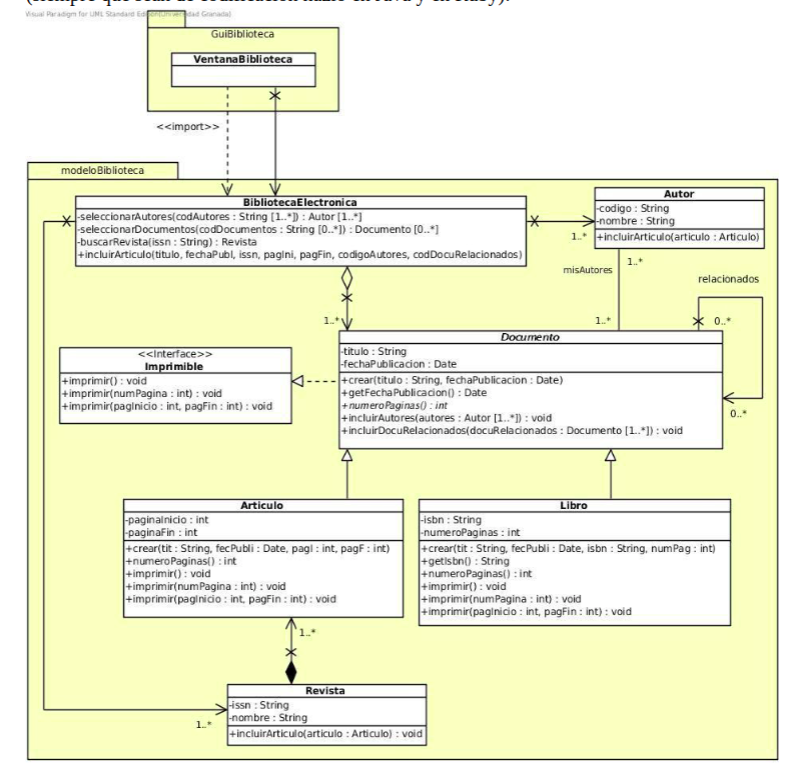
\includegraphics[width=1.1\textwidth]{images/ej13.png}
    \caption{Diagrama de clases}
    \label{fig:ejercicio13}
\end{figure}



\begin{itemize}
    \item Define la clase Documento (cabecera, atributos y cabeceras de los métodos).
    \item Define la clase Articulo (cabecera, atributos y cabeceras de los métodos).
    \item Implementa el constructor que se indica en la clase Artículo.
    \item Define la interfaz Imprimible.
    \item Indica los atributos que definen el estado de la clase BibliotecaElectronica.
    \item La clase Documento figura en cursiva, lo que indica que es abstracta. Indica los dos motivos por los que lo es.
    \item En este modelo, ¿puede haber artículos que no estén ligados a una revista?
    \item Indica sobre las relaciones del diagrama de clases con cuál de los siguientes tipos se corresponden: asociación (AS), agregación (AG), composición (C), realización (R), herencia (H), dependencia (D).
    \item Escribe el contenido del fichero VentanaBiblioteca completo (pero sin añadir nada que no aparezca en el diagrama).
    \item En la clase Articulo, indica cuáles de sus métodos están sobrecargados o redefinidos. Justifica tu respuesta.
    \item Corrige el código:
    \begin{lstlisting}[style=customjava]
    Imprimible docu = new Documento("Intemperie", fecha); // suponiendo que fecha está inicializada
    docu.imprimir();
    \end{lstlisting}
    \item Corrige el código:
    \begin{lstlisting}[style=customjava]
    Documento docu = new Libro("ISBN10102030");
    String codigo = docu.getIsbn();
    \end{lstlisting}
    \item Rellena la siguiente tabla indicando el tipo estático y dinámico de la variable docu en las siguientes líneas de código:
    \begin{table}[H]
        \centering
        \begin{tabular}{|l|l|l|}
            \hline
            \textbf{Código} & \textbf{Tipo estático} & \textbf{Tipo dinámico} \\ \hline
            Documento docu = new Articulo(titulo, fecha, pagIni, pagFin); &  &  \\ \hline
            docu.imprimir(pagIni, pagFin); &  &  \\ \hline
            docu = new Libro(titulo, fecha, isbn, pags); &  &  \\ \hline
            docu.imprimir(); &  &  \\ \hline
        \end{tabular}
    \end{table}
    \item Indica si hay errores de compilación o ejecución en el código anterior (suponiendo que las variables titulo, fecha, pagIni, pagFin, isbn y pags han sido declaradas e inicializadas convenientemente con anterioridad). Justifica tu respuesta.
    \item Rellena la siguiente tabla marcando con una “X” la situación que corresponda a cada una de las líneas del siguiente bloque de código (suponiendo que las variables titulo, fecha, pagIni y pagFin han sido declaradas e inicializadas convenientemente con anterioridad).
    \begin{table}[H]
        \centering
        \begin{tabular}{|p{4cm}|p{4cm}|p{4cm}|p{4cm}|}
            \hline
            \textbf{Código} & \textbf{Ningún error} & \textbf{Sólo error de compilación} & \textbf{Sólo error de ejecución} \\ \hline
            Imprimible imp = new Articulo(titulo, fecha, pagIni, pagFin); &  &  &  \\ \hline
            Documento docu = imp; &  &  &  \\ \hline
            imp.numeroPaginas(); &  &  &  \\ \hline
            ((Libro) docu).getIsbn(); &  &  &  \\ \hline
        \end{tabular}
    \end{table}
\end{itemize}

\subsection{Solución en Java}

\begin{lstlisting}[style=customjava, caption={lase Documento (cabecera, atributos y cabeceras de los métodos)}]
    abstract class Documento implements Imprimible{
        private String titulo;
        private Date fechaPublicacion;
        private Autor misAutores[];
        private Documento relacionados[];


        public Documento(String titulo, Date fechaPublicacion);

        public Date getFechaPublicacion();

        public abstract int numeroPaginas();

        public void public incluirAutores(Autor[] autores);

        public void incluirDocuRelacionados(Documento[] docuRelacionados);


    }

\end{lstlisting}

\begin{lstlisting}[style=customjava, caption={clase Articulo (cabecera, atributos y cabeceras de los métodos), constructor de la clase Artículo}]
    class Articulo extends Documento{
        private int paginaInicio;
        private int paginaFin;

        public Articulo(String tit, Date fecPubli, int pagI, int pagF){
            super(tit, fecPubli);
            this.paginaInicio = pagI;
            this.paginaFin = pagF;
        }
        public int numeroPaginas();
        public void imprimir();
        public void imprimir(int numeroPagina);
        public void imprimir(int pagInicio, int pagFin);
    }
    
\end{lstlisting}

\begin{lstlisting}[style=customjava, caption = {Intefaz Imprimible}]
    interface Imprimible {
        void imprimir();
        void imprimir(int numeroPagina);
        void imprimir(int pagInicio, int pagFin);
    }



\end{lstlisting}

\begin{lstlisting}[style = customjava, caption = {Atributos que definen el estado de la clase BibliotecaElectronica}]
    class BibliotecaElectronica{
        private Autor autores[];
        private Documento documentos[];
        private Revista resvistas[];
    }
\end{lstlisting}

\subsubsection*{Motivos por los que la clase Documento es abstracta}
\begin{enumerate}
    \item Sirve como clase plantilla para las clases Libro y Revista que son clases hijas según el diagrama de clases.
    \item Contiene al menos un método abstracto, que en este caso es el método \texttt{numeroPaginas()}.
\end{enumerate}

\subsubsection*{¿Puede haber artículos que no estén ligados a una revista?}

En este modelo si, lo que no puede haber son revistas que no estén ligadas a un Artículo debido al diagrama de clases y la lógica del rombo de la flecha de composición de la clase Artículo (parte de esta).

\subsubsection*{Pintar en el diagrama de clases las uniones de: asociación (AS), agregación (AG), composición (C), realización (R), herencia (H), dependencia (D)}

\begin{figure}[H]
    \centering
    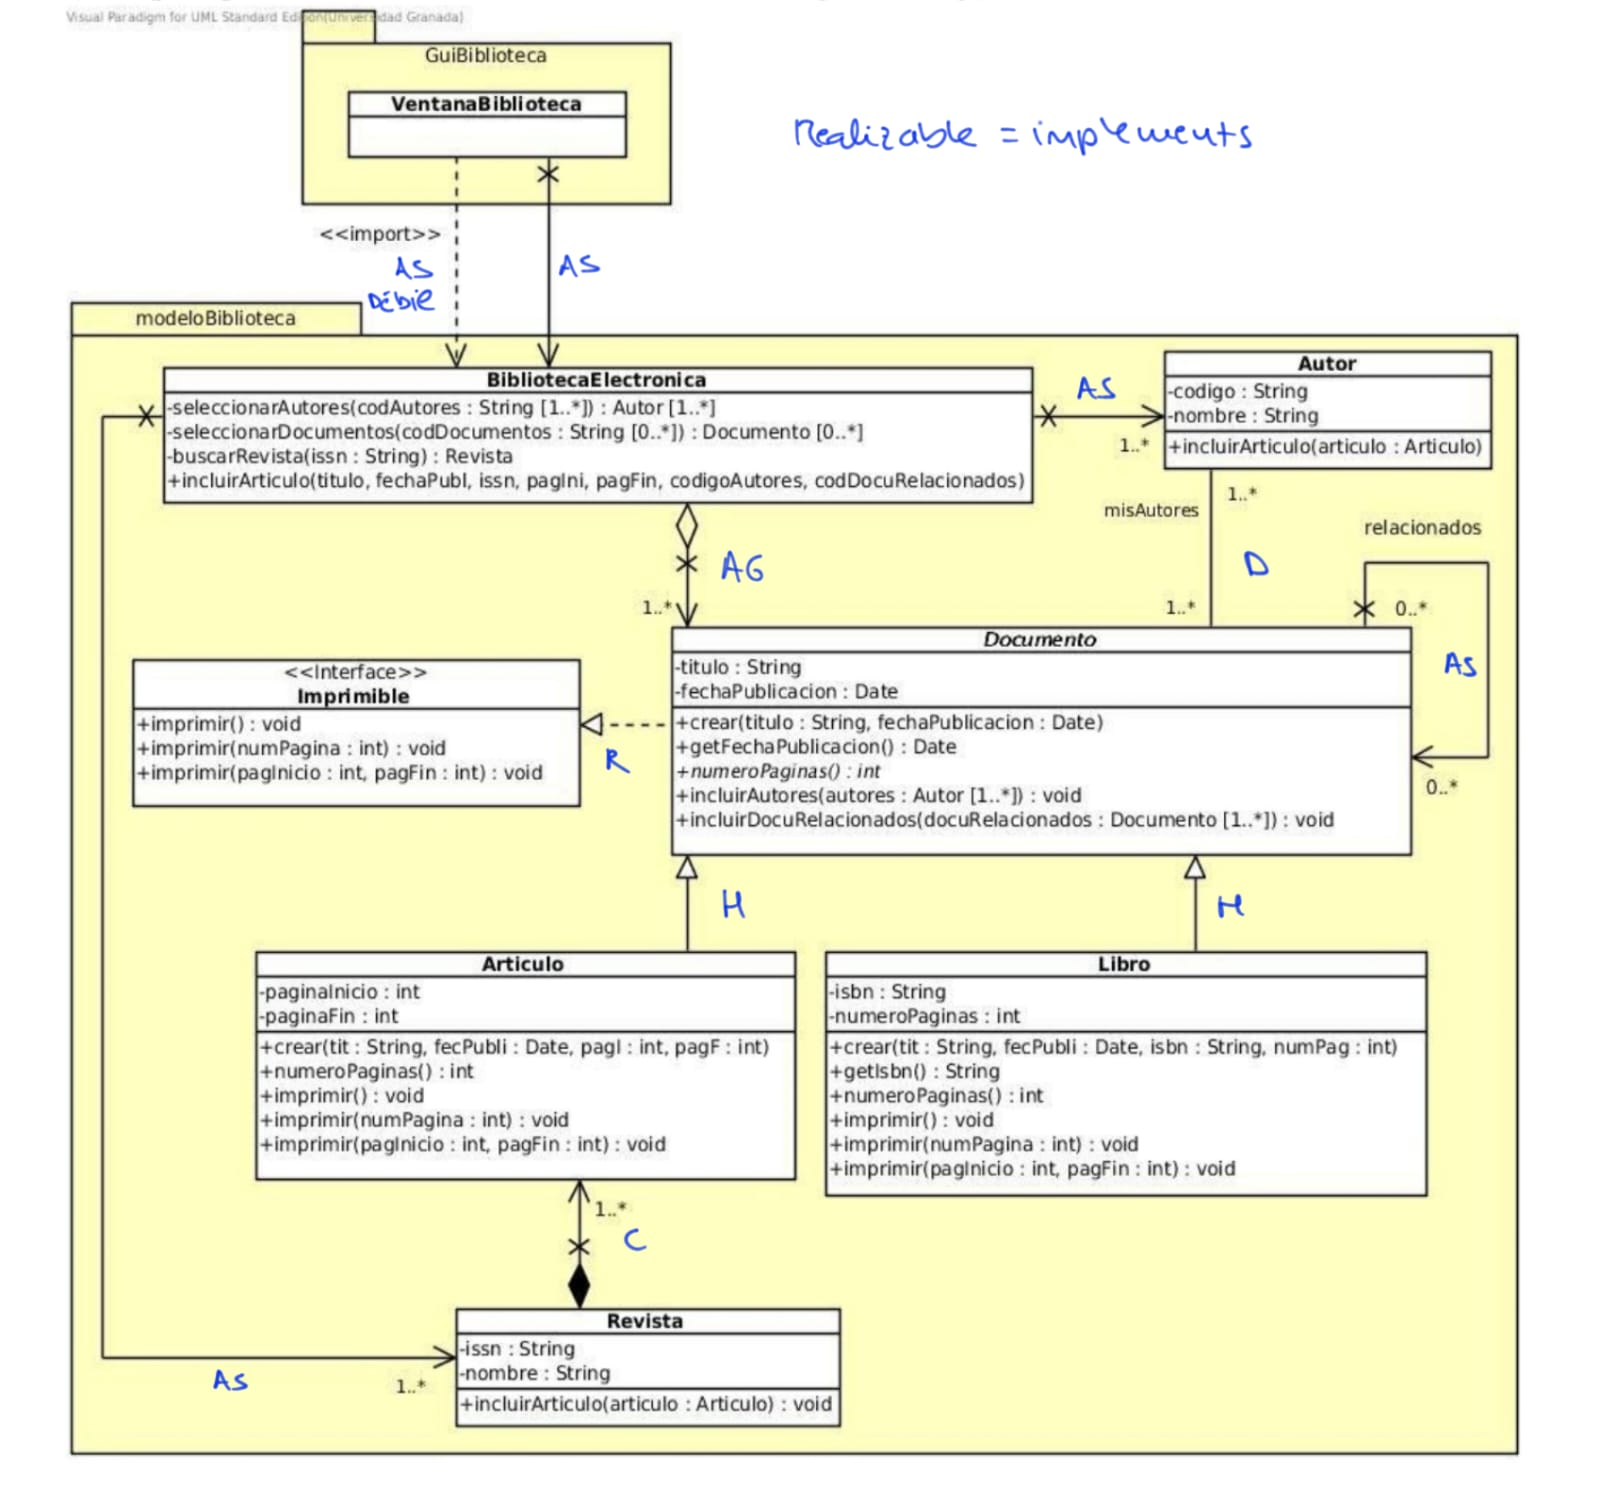
\includegraphics[width=0.9\textwidth]{images/ej12.png}
    \caption{Diagrama de clases}
    \label{fig:ejercicio12}
\end{figure}

\subsubsection*{Contenido del fichero VentanaBiblioteca completo (pero sin añadir nada que no aparezca en el diagrama)}

\begin{lstlisting}[style=customjava, caption={VentanaBiblioteca, el constructor se puede obviar, ya que usaríamos el por defecto}]
    class VentanaBiblioteca{
        private BibliotecaElectronica biblioteca;

        public VentanaBiblioteca(BibliotecaElectronica biblioteca){
            this.biblioteca = biblioteca;
        }
    }
\end{lstlisting}

\subsubsection*{En la clase Articulo, indica cuáles de sus métodos están sobrecargados o redefinidos. Justifica tu respuesta.}

\begin{itemize}
    \item El método \texttt{imprimir()} está redefinido porque aparece en la clase \texttt{Documento}, el cual lo implementa de la interfaz \texttt{Imprimible}.
    \item El método \texttt{imprimir(int numeroPagina)} está redefinido porque aparece en la clase \texttt{Documento}, el cual lo implementa de la interfaz \texttt{Imprimible}.
    \item El método \texttt{imprimir(int pagInicio, int pagFin)} está redefinido porque aparece en la clase \texttt{Documento}, el cual lo implementa de la interfaz \texttt{Imprimible}.
    \item El método \texttt{numeroPaginas()} está redefinido porque sobrescribe el método de la clase \texttt{Documento}. Aunque sea abstracto, al cambiar únicamente el tipo se considera una redefinición\footnote{Mirar ejercicio 1.}.
\end{itemize}

\subsubsection*{Corrige el código}

    \begin{lstlisting}[style=customjava, caption = {Código a corregir}]
    Imprimible docu = new Documento("Intemperie", fecha); // suponiendo que fecha está inicializada
    docu.imprimir();
    \end{lstlisting}

Corrección:
\begin{lstlisting}[style=customjava, caption={Corrección del código}]
    Documento docu = new Articulo("Intemperie", fecha, 1, 10);
    docu.imprimir();
\end{lstlisting}

\subsubsection*{Corrige el código:}
    \begin{lstlisting}[style=customjava, caption = {Código a corregir}]
    Documento docu = new Libro("ISBN10102030");
    String codigo = docu.getIsbn();
    \end{lstlisting}

Corrección:
\begin{lstlisting}[style=customjava, caption={Corrección del código}]
    Libro docu = new Libro("ISBN10102030");
    String codigo = docu.getIsbn();
\end{lstlisting}

\subsubsection*{Rellena la siguiente tabla indicando el tipo estático y dinámico de la variable docu en las siguientes líneas de código:
}    
    \begin{table}[H]
        \centering
        \begin{tabular}{|p{6cm}|l|l|}
            \hline
            \textbf{Código} & \textbf{Tipo estático} & \textbf{Tipo dinámico} \\ \hline
            Documento docu = new Articulo(titulo, fecha, pagIni, pagFin); & Documento & Articulo \\ \hline
            docu.imprimir(pagIni, pagFin); & Documento & Articulo \\ \hline
            docu = new Libro(titulo, fecha, isbn, pags); & Documento & Libro \\ \hline
            docu.imprimir(); & Documento & Libro \\ \hline
        \end{tabular}
    \end{table}


\subsubsection*{Indica si hay errores de compilación o ejecución en el código anterior (suponiendo que las variables titulo, fecha, pagIni, pagFin, isbn y pags han sido declaradas e inicializadas convenientemente con anterioridad). Justifica tu respuesta.}

\begin{itemize}
    \item En la primera línea de código no hay errores de compilación ni de ejecución.
    \item Si, debido a que no puedes usar imprimir de Documento, ya que aunque derive de la interfaz que lo tenga, no esta implementado en Documento. Vemos que esta en Artículo, pero para usarlo debemos de realizar un cast: \texttt{((Articulo)docu).imprimir();} \textit{Nota: en java solo se puedes usar las funciones de los tipos estáticos, por eso en este caso da error de compilación y lo tenemos que hacer de la manera indicada.}
    \item En la tercera línea de código no hay errores de compilación ni de ejecución.
    \item Pasa lo mismo que en la 2º explicación de este.
\end{itemize}

\subsubsection*{Rellena la siguiente tabla marcando con una “X” la situación que corresponda a cada una de las líneas del siguiente bloque de código (suponiendo que las variables titulo, fecha, pagIni y pagFin han sido declaradas e inicializadas convenientemente con anterioridad).}

\begin{table}[H]
    \centering
    \begin{tabular}{|p{4cm}|p{4cm}|p{4cm}|p{4cm}|}
        \hline
        \textbf{Código} & \textbf{Ningún error} & \textbf{Sólo error de compilación} & \textbf{Sólo error de ejecución} \\ \hline
        Imprimible imp = new Articulo(titulo, fecha, pagIni, pagFin); & X &  &  \\ \hline
        Documento docu = imp; &  & X &  \\ \hline
        imp.numeroPaginas(); &  & X &  \\ \hline
        ((Libro) docu).getIsbn(); &  &  & X \\ \hline
    \end{tabular}
\end{table}

\subsection{Solución en Ruby}

\begin{lstlisting}[style=customrb, caption={Clase Documento (cabecera, atributos y cabeceras de los métodos)}]
    class Documento
        attr_reader :titulo, :fecha_publicacion

        def initialize(titulo, fecha_publicacion)
            @titulo = titulo
            @fecha_publicacion = fecha_publicacion
        end

        def numero_paginas
            raise NotImplementedError, 'Debe ser implementado en una subclase'
        end

        def incluir_autores(autores)
            # Implementación
        end

        def incluir_documentos_relacionados(documentos)
            # Implementación
        end
    end
\end{lstlisting}

\begin{lstlisting}[style=customrb, caption={Clase Articulo (cabecera, atributos y cabeceras de los métodos), constructor de la clase Artículo}]
    class Articulo < Documento
        attr_reader :pagina_inicio, :pagina_fin

        def initialize(titulo, fecha_publicacion, pagina_inicio, pagina_fin)
            super(titulo, fecha_publicacion)
            @pagina_inicio = pagina_inicio
            @pagina_fin = pagina_fin
        end

        def numero_paginas
            @pagina_fin - @pagina_inicio + 1
        end

        def imprimir
            # Implementación
        end

        def imprimir_por_pagina(numero_pagina)
            # Implementación
        end

        def imprimir_por_rango(pagina_inicio, pagina_fin)
            # Implementación
        end
    end
\end{lstlisting}

\begin{lstlisting}[style=customrb, caption={Interfaz Imprimible}]
    module Imprimible
        def imprimir
            # Implementación
        end

        def imprimir_por_pagina(numero_pagina)
            # Implementación
        end

        def imprimir_por_rango(pagina_inicio, pagina_fin)
            # Implementación
        end
    end
\end{lstlisting}

\begin{lstlisting}[style=customrb, caption={Atributos que definen el estado de la clase BibliotecaElectronica}]
    class BibliotecaElectronica
        attr_accessor :autores, :documentos, :revistas
    end
\end{lstlisting}





\section{Ejercicio 13}

\begin{figure}[H]
    \centering
    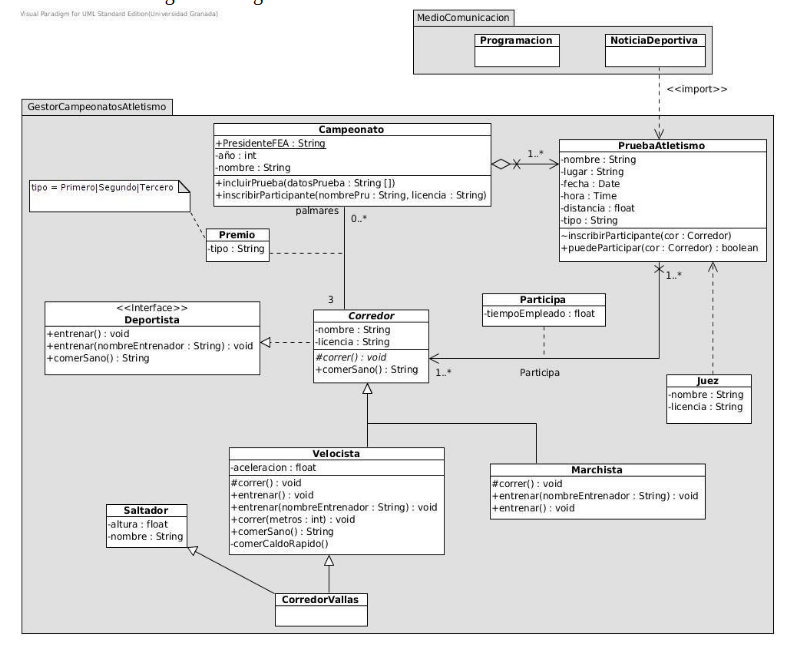
\includegraphics[width=1.1\textwidth]{images/ej14.png}
    \caption{Diagrama de clases}
    \label{fig:ejercicio14}
\end{figure}

\subsection{Enunciado Y Solución}

%tabla 1
\begin{table}[H]
    \centering
    \begin{tabular}{|p{7cm}|c|}
    \hline
    \textbf{Cuestión} & \textbf{Respuesta} \\ \hline
    Desde la clase NoticiaDeportiva se puede acceder a todos los elementos públicos del paquete GestorCampeonatosAtletismo directamente & F \\ \hline
    Un CorredorVallas es un Velocista y Saltador & V \\ \hline
    El estado de un objeto de la clase Juez no viene determinado por el estado de un objeto de la clase PruebaAtletismo & V \\ \hline
    Una PruebaAtletismo puede existir sin estar asociada a la clase Campeonato & V \\ \hline
    Un Velocista es un Corredor & V \\ \hline
    Un Deportista es un Corredor & F \\ \hline
    La clase Corredor tiene 4 métodos, 3 abstractos y 1 concreto & F \\ \hline
    La clase Marchista está mal representada en el diagrama, debe ser abstracta & F \\ \hline
    La clase CorredorVallas presenta un conflicto de nombres & F \\ \hline
    Todas las instancias de la clase Campeonato tienen una copia de la variable PresidenteFEA & V \\ \hline
    \end{tabular}
    \caption{Cuestiones Verdaderas o Falsas}
\end{table}

%tabla2
% Tabla de métodos abstractos en Marchista
\begin{table}[H]
    \centering
    \begin{tabular}{|l|c|}
    \hline
    \textbf{Método} & \textbf{Abstracto} \\ \hline
    correr() & No, porque es una redefinición de Corredor  \\ \hline
    comerSano() &   No, es una redefinición de la clase Corredor \\ \hline
    entrenar() &   No, porque es una redefinición de la interfaz Deportista \\ \hline
    entrenar(nombreEntrenador:String) &  No, porque es una redefinición de la interfaz Deportista \\ \hline
    \end{tabular}
    \caption{Métodos abstractos en Marchista}
\end{table}

% Tabla de métodos redefinidos y sobrecargados en Velocista
\begin{table}[H]
    \centering
    \begin{tabular}{|l|c|c|}
    \hline
    \textbf{Método} & \textbf{Redefinido} & \textbf{Sobrecargado} \\ \hline
    correr() & X, porque cambia la cabecera &  \\ \hline
    comerSano() & X &  \\ \hline
    entrenar() & X, aunque sea de la interfaz &  \\ \hline
    \end{tabular}
    \caption{Métodos redefinidos o sobrecargados en Velocista}
\end{table}

% Tabla de tipo estático y dinámico de variables
\begin{table}[H]
    \centering
    \begin{tabular}{|l|l|l|l|}
    \hline
    & \textbf{Variable} & \textbf{Tipo Estático} & \textbf{Tipo Dinámico} \\ \hline
    Deportista c = new Velocista(); & c& Deportista & Velocista \\ \hline
    Corredor d = new Marchista(); &d &Corredor & Marchista \\ \hline
    c = new Marchista(); &c& Deportista & Marchista \\ \hline
    d = c; & d&Corredor & Marchista \\ \hline
    \end{tabular}
    \caption{Tipo estático y dinámico de variables}
\end{table}

%ultima parte
\begin{table}[H]
    \centering
    \begin{tabular}{|p{7cm}|p{5cm}|p{3cm}|}
        \hline
        \textbf{Código} & \textbf{Corrección del error en Compilación} & \textbf{Error en ejecución} \\ \hline
        Corredor c = new Velocista(); & Ninguno & Ninguno \\ \hline
        Deportista d = new Marchista(); & Ninguno & Ninguno \\ \hline
        d.comerSano(); & Ninguno & Ninguno \\ \hline
        Marchista m = (Marchista) d; & Ninguno & Ninguno \\ \hline
        d = c; & Ninguno & Ninguno \\ \hline
        d.correr(150); & El método correr(int) no está definido en la interfaz Deportista & Ninguno \\ \hline
        Velocista v = (Velocista) d; & Ninguno & Error en ejecución si d no es una instancia de Velocista \\ \hline
        ArrayList<Corredor> corredores = new ArrayList<>(); & Ninguno & Ninguno \\ \hline
        corredores.add(c); & Ninguno & Ninguno \\ \hline
        corredores.add(m); & Ninguno & Ninguno \\ \hline
        corredores.get(0).correr(10); & El método correr(int) no está definido en Corredor & Ninguno \\ \hline
        corredores.get(1).correr(10); & El método correr(int) no está definido en Corredor & Ninguno \\ \hline
        c = new Corredor(); & No se puede instanciar una clase abstracta & Ninguno \\ \hline
    \end{tabular}
    \caption{Corrección de errores de compilación y ejecución}
\end{table}

Para una explicación más detallada pincha \href{https://github.com/ElblogdeIsmael/ElblogdeIsmael.github.io/tree/main/Asignaturas/Tercer%20A%C3%B1o/PDOO/Teoria/RelacionesEjercicios/Solt3/ETSIIT/explicacion_ej14.md}{aquí}.

%codigo
\begin{lstlisting}[style=customjava, caption={Código en java}]
    public class Club<T> {
    private Map<String, T> miembros; // key = número de licencia
    private T lider;

    // Constructor
    public Club(T lider) {
        this.lider = lider;
        this.miembros = new HashMap<>();
    }

    // Consultor de un miembro del club a partir del numero de licencia
    public T getMiembro(String numeroLicencia) {
        return miembros.get(numeroLicencia);
    }

    // Incluir un nuevo miembro en el club
    public void incluirMiembro(String numeroLicencia, T miembro) {
        miembros.put(numeroLicencia, miembro);
    }

    // Cambiar el líder
    public void setLider(T lider) {
        this.lider = lider;
    }

    // Obtener el líder
    public T getLider() {
        return lider;
    }
}
\end{lstlisting}

\begin{lstlisting}[style=customcpp, caption={Main}]
import java.util.HashMap;
import java.util.Map;

public class Main {
    public static void main(String[] args) {
        // Creamos una instancia de Velocista
        Velocista lider = new Velocista("Usain Bolt", "001", 9.58f);

        // Creamos un club de Velocistas, con Usain Bolt como líder inicial
        Club<Velocista> clubDeVelocistas = new Club<>(lider);

        // Creamos más miembros del club
        Velocista miembro1 = new Velocista("Carl Lewis", "002", 9.86f);
        Velocista miembro2 = new Velocista("Tyson Gay", "003", 9.69f);

        // Añadimos miembros al club
        clubDeVelocistas.incluirMiembro("002", miembro1);
        clubDeVelocistas.incluirMiembro("003", miembro2);

        // Consultamos los miembros
        System.out.println("Líder del club: " + clubDeVelocistas.getLider().getNombre());
        System.out.println("Miembro con licencia 002: " + clubDeVelocistas.getMiembro("002").getNombre());
        System.out.println("Miembro con licencia 003: " + clubDeVelocistas.getMiembro("003").getNombre());

        // Cambiamos el líder del club
        clubDeVelocistas.setLider(miembro1);
        System.out.println("Nuevo líder del club: " + clubDeVelocistas.getLider().getNombre());
    }
}

// Clase Velocista
class Velocista {
    private String nombre;
    private String licencia;
    private float mejorMarca;

    // Constructor
    public Velocista(String nombre, String licencia, float mejorMarca) {
        this.nombre = nombre;
        this.licencia = licencia;
        this.mejorMarca = mejorMarca;
    }

    // Getters
    public String getNombre() {
        return nombre;
    }

    public String getLicencia() {
        return licencia;
    }

    public float getMejorMarca() {
        return mejorMarca;
    }
}

\end{lstlisting}

\begin{lstlisting}[caption = {Salida del Main}]
Líder del club: Usain Bolt
Miembro con licencia 002: Carl Lewis
Miembro con licencia 003: Tyson Gay
Nuevo líder del club: Carl Lewis

\end{lstlisting}


\section{Ejercicio 14}

\subsection{Enunciado}

Dado el siguiente diagrama de clases:
\begin{figure}[H]
    \centering
    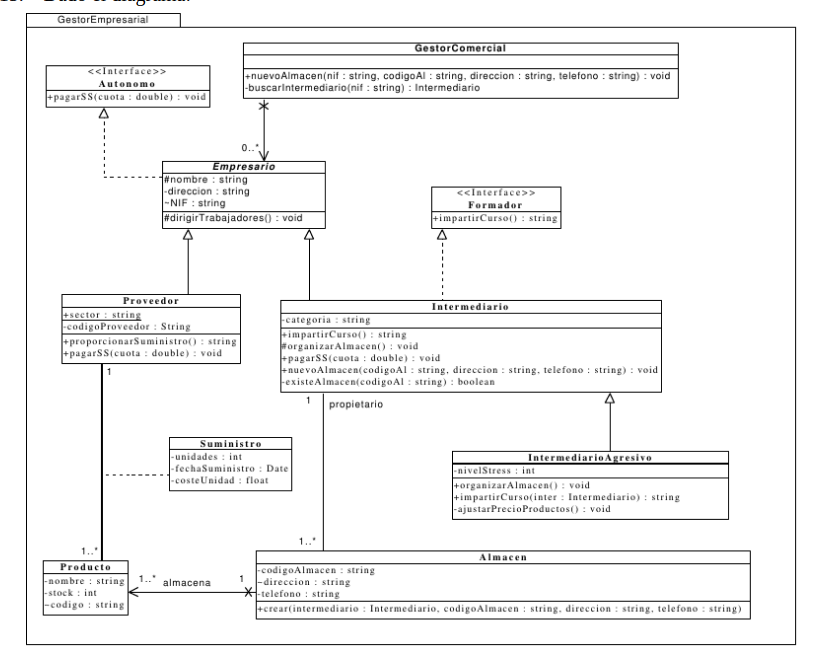
\includegraphics[width=1.1\textwidth]{images/ej15.png}
    \caption{Diagrama de clases}
    \label{fig:ejercicio15}
\end{figure}


Indica si las siguientes líneas de código Java producen error de compilación, de ejecución, ambos o ninguno. Supón que están en un \texttt{main} en una clase nueva dentro del mismo paquete. Si hay error explica cómo lo arreglarías y si no hay error, indícalo explícitamente. Considera para este ejercicio que todas las clases tienen un constructor válido que no recibe atributos.

\begin{table}[H]
    \centering
    \begin{tabular}{|l|p{2.5cm}|p{2cm}|}
        \hline
        \textbf{Código} & \textbf{Error de compilación} & \textbf{Error de ejecución} \\ \hline
        Formador f = new Intermediario(); & Ninguno & Ninguno \\ \hline
        f.pagarSS(23.4); & Ninguno & Ninguno \\ \hline
        Autonomo auto1 = f; & Sí & Ninguno \\ \hline
        Autonomo auto2 = (Proveedor) f; & Sí & Ninguno \\ \hline
        IntermediarioAgresivo emp1 = new IntermediarioAgresivo(); & Ninguno & Ninguno \\ \hline
        emp1.ajustarPrecioProductos(); & Ninguno & Ninguno \\ \hline
        Empresario emp2 = new Empresario(); & Ninguno & Ninguno \\ \hline
        ArrayList<Formador> formadores = new ArrayList(); & Sí & Ninguno \\ \hline
        formadores.add(f); & Ninguno & Ninguno \\ \hline
        formadores.add(emp1); & Ninguno & Ninguno \\ \hline
        formadores.get(1).impartirCurso(); & Ninguno & Ninguno \\ \hline
        formadores.get(1).impartirCurso(f); & Sí & Ninguno \\ \hline
        ((IntermediarioAgresivo)formadores.get(0)).impartirCurso(emp1); & Ninguno & Ninguno \\ \hline
    \end{tabular}
\end{table}

\subsection{Solución}

\begin{table}[H]
    \centering
    \begin{tabular}{|l|p{2.5cm}|p{2 cm}|}
        \hline
        \textbf{Código} & \textbf{Error de compilación} & \textbf{Error de ejecución} \\ \hline
        Formador f = new Intermediario(); & Ninguno & Ninguno \\ \hline
        f.pagarSS(23.4); & Ninguno & Ninguno \\ \hline
        Autonomo auto1 = f; & Sí & Ninguno \\ \hline
        Autonomo auto2 = (Proveedor) f; & Sí & Ninguno \\ \hline
        IntermediarioAgresivo emp1 = new IntermediarioAgresivo(); & Ninguno & Ninguno \\ \hline
        emp1.ajustarPrecioProductos(); & Ninguno & Ninguno \\ \hline
        Empresario emp2 = new Empresario(); & Ninguno & Ninguno \\ \hline
        ArrayList<Formador> formadores = new ArrayList(); & Sí & Ninguno \\ \hline
        formadores.add(f); & Ninguno & Ninguno \\ \hline
        formadores.add(emp1); & Ninguno & Ninguno \\ \hline
        formadores.get(1).impartirCurso(); & Ninguno & Ninguno \\ \hline
        formadores.get(1).impartirCurso(f); & Sí & Ninguno \\ \hline
        ((IntermediarioAgresivo)formadores.get(0)).impartirCurso(emp1); & Ninguno & Ninguno \\ \hline
    \end{tabular}
\end{table}


Para una explicación más detallada pincha \href{https://github.com/ElblogdeIsmael/ElblogdeIsmael.github.io/tree/main/Asignaturas/Tercer%20A%C3%B1o/PDOO/Teoria/RelacionesEjercicios/Solt3/ETSIIT/explicacion_ej15.md}{aquí}.



\end{document}